\documentclass[oneside,numberorder]{tjmath}
%还有twoside选项,可以添加,类似book里的twoside
%TODO:完善twoside选项
\usepackage{lastpage}
\usepackage{url}

\DeclareMathOperator*{\argmin}{arg\,min}
\DeclareMathOperator*{\argmax}{arg\,max}
%可以自己添加数学类的操作符,这里只是举例

\begin{document}
  %\tjutitle{题目中文名}{题目英文名}
	\tjutitle{股票挂钩型理财产品的定价模型及金融分析}{Pricing model of stock-linked financial products and financial analysis}
  %\tjuauthor{中文名}{英文名}{学号}
	\tjuauthor{李冰冰}{Binging Lee}{083666}
  %\tjumentor{导师中文名}{导师英文名}
	\tjumentor{张忠良}{Zhang.Z.L}
  %\tjuinfo{年级}{专业名}
	\tjuinfo{2009级}{数学与应用数学}
  %\tjucollege{系中文名}{系英文名}
	\tjucollege{数学系}{Math Department}
  %之所以要输入英文名,是为了twoside里的英文封面做准备 TODO


  %封面信息,可以在data文件夹下的cover.tex文件中自行修改样式,内容部分不用修改
	%======================================
%%封面
%======================================
\thispagestyle{empty}

\vspace{10mm}

\begin{center}
	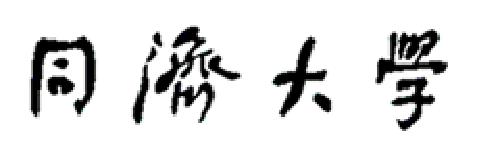
\includegraphics[width=108mm]{pic/logo}
\end{center}

\centerline{\songti \erhao \textbf{本\, 科\, 生\, 毕\, 业\, 论\, 文}}
\vspace{8mm}

\begin{center}
	
\includegraphics[width=40mm]{pic/tj}
\end{center}

\vspace{32mm}

\begin{tabbing}
	\hspace{30mm} \= \songti\sihao 学生姓名: \=\underline{\makebox[6cm]{\sihao\tjuauthornamec} }\\[2mm]
	\>\songti \sihao 学生学号:\> \underline{\makebox[6cm]{\sihao \tjuauthorid}} \\[2mm]
	\>\songti \sihao 指导教师:\> \underline{\makebox[6cm]{\sihao \tjumentorc}}\\[2mm]
	\> \songti\sihao 专\hspace{10mm}业: \> \underline{\makebox[6cm]{\sihao\tjugrade\hspace{3mm}\tjumajor}} \\[2mm]
	\>\songti \sihao 学\hspace{10mm}院:\> \underline{\makebox[6cm]{\sihao \tjucollegec}}
\end{tabbing}

%======================================
%双面设置
%======================================
\ifthenelse{\equal{\tjuside}{T}}{
	\newpage\mbox{}
	\thispagestyle{empty}}{}





  %申明部分,可以在data文件夹下的announce.tex文件中自行修改
  \newpage
\thispagestyle{empty}

\begin{center}
	\heiti\xiaosan 同济大学本科生毕业设计(论文)诚信承诺书
\end{center}

\vspace{5mm}

{\songti\sihao
\begin{enumerate}
	\item 本人郑重地承诺所呈交的毕业设计(论文),是在指导教师的指导下严格按照学校和学院有关规定完成的。
	\item 本人承诺毕业设计(论文)选题和研究内容过程中没有抄袭他人研究成果和伪造相关数据等行为。
	\item 在毕业设计(论文)中对侵犯任何方面知识产权的行为,由本人承担相应的法律责任。
\end{enumerate}
\vspace{20mm}
\hspace{20mm}毕业设计(论文)作者签名:
\begin{flushright}
	\underline{\hspace{4em}} 年 \underline{\hspace{2em}}月\underline{\hspace{2em}}日
\end{flushright}
}


  \frontmatter
  \pagenumbering{Roman}
    %中文摘要部分,英文部分可以自己添加
  	\chapter*{\centerline{\tjutitlec}}
\chaptermark{摘要}
\addcontentsline{toc}{chapter}{摘要}

\vspace{1em}
\noindent{\songti \xiaowu【摘要】\quad 文章给给出一个招商银行的股票挂钩型理财产品,先简化模型,减少股票数量,在每个记息期上利用欧式期权的Black-Scholes 公式,建立单资产模型,逐段求解,给出解析解。然后再对其还原,建立3支股票的多资产模型并求解,给出了3只股票情况下的多资产模型的解析解,然后将1维和3维情况下的解析解进行比较,互相检验。最后利用真实的股票数据对简化的单资产模型进行模拟,定价,并画图形,最后在画出此金融产品价值与各个参数之间的图形。}

\vspace{1em}
\noindent{\songti \xiaowu 【关键词】 \quad  股票挂钩型理财产品 \quad 期权定价 \quad 多资产期权} 


  	\tableofcontents
  	\chaptermark{目录}
    \addcontentsline{toc}{chapter}{目录}

  	\mainmatter
%========================装订线部分,待测试===========================
    %\setlength{\unitlength}{1mm}
    %\begin{picture}(10,30)
    %\put(-20,-180){\shortstack[c]{ %第一个负号向左移,第二个负向下移
    %| \\ | \\| \\| \\| \\| \\| \\ 装\\
    %| \\ | \\| \\| \\| \\| \\| \\ 订\\
    %| \\ | \\| \\| \\| \\| \\| \\ 线\\
    %| \\ | \\| \\| \\| \\| \\| }}
    %\end{picture}
%TODO


 %=========================正文部分开始=================================

    \chapter{前言}

\section{股票挂钩型理财产品}

股票挂钩投资品,又称连动式投资产品或结构型投资产品,是一种收益与股票价格或股价指数等标的相挂钩的结构化产(Structure Products)。通过财务工程技术,针对投资者对市场之不同预期,以拆解或组合衍生性金融商品如股票、一篮子股票、指数、一篮子指数等,并搭配零息债券的方式组合而成的各种不同报酬型态的金融商品。\cite{optionpricing}

\section{挂钩型理财产品市场现状}

挂钩型理财产品发展历史不长,但发展极为迅速,已实现在美国证券交易所、伦敦证券交易所、香港联交易所等处上市交易,是当今国际金融市场上最有发展潜力的业务之一。目前,此类产品已开始中国境内销售,有望成为优良的理财产品以及权证的背对产品,市场前景可观。\cite{On-Manifold-Regularization}

挂钩股指,如汇丰银行此前发行的新品则挂钩股指的绝对值,只要其对应的恒生中国企业指数波动达到一定的幅度,投资者就能获得相应的回报。

在挂钩范围上,此类产品的选择也越来越多,不断有新的热点涌现。如荷兰银行推出的挂钩房地产股票篮子以及水资源股票的产品、渣打银行挂钩媒体篮子股票的产品以及最近民生银行推出的挂钩香港中国概念金融板块股票的非凡人民币理财产品等,使得挂钩股票型产品的投资方向日渐多样化。有些产品的收益相当不错,如荷兰银行去年6月推出的第一期挂钩房地产股票篮子的结构性产品,截至11月2日,该产品的美元和欧元的收益率已分别达到12\%和8\% 。

与市场上越来越多的短期理财产品相比,挂钩股票型的理财产品投资期限普遍较长,大部分产品的投资期限都是在2年左右。这主要是由产品挂钩股票的特点所决定的,时间太短,一旦股价出现较大的波动,不但不能给投资者带来收益,反而会带来损失。因此一段较长的投资期限是获取收益、平摊风险的必需条件。另一方面,银行在发行挂钩股票型产品时都承诺本金的保证,但前提是投资者必须要持有理财计划到期,否则本金就会有损失。

\section{期权}
\subsection{期权的概念}
期权是20世纪70年代中期在美国出现的一种金融创新工具,30多年来,它作为一种防范风险和投机的有效手段而得到迅猛发展。

期权是一种极为特殊的衍生产品,它能使买方有能力避免坏的结果,而从好的结果中获益,同时.它也能使卖方产生巨大的损失。当然,期权不是免费的,这就产生了期权定价问题。期权定价理论是现代金融理论最为重要的成果之一。\cite{optionpricing}它集中体现了金融理论的许多核心问题,其理论之深,方法之多,应用之广,令人惊叹。期权的标的资产也由股票、指数、期货台约、商品(金属、黄金、石油等),外汇增加到了利率,可转换债券、认股权证、掉期和期权本身等许多可交易证券和不可交易证券.期权是一种企业、银行和投资者等进行风险管理的有力工具。

\subsection{期权和期权理论的历史}
期权的理论与实践并非始于1973年Black-Scholes关于期权定价理论论文的发表。早在公元前1200年的古希腊和古腓尼基国的贸易中就已经出现了期权交易的雏形,只不过当时条件下不可能对其有深刻认识。期权的思想萌芽也可以追溯到公元前1800年的《汉穆拉比法典》。公认的期权定价理论的始祖是法国数学家巴舍利耶 (LouisBachelier,1900年)。令人难以理解的是.长达半个世纪之久巴舍利耶的工作没有引起金融界的重视,直到l956年被克鲁辛格(Kruizenga)再次发现。\cite{kexuebao}


    \chapter{Black-Scholes方程的假设以及研究对象的分析}

\section{B-S方程的假设}
从73年美国芝加哥大学学者提出B-S 期权定价模型以来,各种新型期权纷纷涌现,但是不管怎样变化都是万变不离其宗,基于基本的B-S方程。当然,B-S 方程并不能完全符合金融市场中的实际情况,但是它的定价理论能够在下述假设下,较真实地反映期权应该具备的价值,并直接应用于金融机构对各种期权的定价。
\begin{tjuhypothsis}
	原生资产价格演化遵循几何Brown运动,即满足如下方程:
	\begin{displaymath}
		dS=\mu Sdt+\sigma SdW
	\end{displaymath}
	$\mu$----期望回报率(常数)\\
	$\sigma$----波动率(常数)\\
	$dW$----标准Brown运动
	\begin{displaymath}
		E(dW)=0
	\end{displaymath}
	$$ Var(dW)=dt $$
\end{tjuhypothsis}
\begin{tjuhypothsis}
	没有交易费用或税收。在现实的金融市场中交易费用和税收都是无法避免的,可是由于许多期权都是大额交易,相对而言,这些费用可以在一定程度上不予考虑。
\end{tjuhypothsis}
\begin{tjuhypothsis}
	市场是公平的、透明的,不存在无风险套利机会。虽然金融市场趋于完善,但是即便在金融业极度发达的国家,无风险套利机会都还是存在的。由于人们都是很理性的,这种套利机会一旦出现立刻被大众所得,根据供求平衡理论可以理解,套利机会会在出现后的短时间内消失。
\end{tjuhypothsis}
\begin{tjuhypothsis}
	原生资产不支付股息。
\end{tjuhypothsis}
\begin{tjuhypothsis}
	无风险利率是常数,即无论到期日为何时,利率均不变。
\end{tjuhypothsis}

\section{研究对象分析}
本文的研究对象为招商银行的股票挂钩型理财产品,该产品与中石油,中移动,中国人寿3支股票挂钩,投资期为2年,认购金额为5万元人民币,每6个月为一个计息期,具有自动终止条款,投资者无权提前终止。这个金融产品是挂钩型理财产品中的保障本金投资产品,并且挂钩3支股票价格,无论票的涨跌,本金都是得到保障的。具体的挂钩股票的条款是:在6个月的观察日,如果3支股票的收盘价格大于或者等于收盘价格的100\%,投资者就可以获得最高的当期理财收益,即:当期理财收益=(理财本金的5\%)/2;如果3支股票的收盘价格大于或者等于收盘价格的95\%,即:当期理财收益=(理财本金的3.5\%)/2;否则,当期收益为0。


    \chapter{期权模型的建立及求解}
\section{单资产模型}
\subsection{记号约定}
\subsection{对此金融产品的简化以及条约分析}
研究对象为招商银行的股票挂钩型理财产品,该产品与中石油,中移动,中国人寿3支股票挂钩,投资期为2年,认购金额为5万元人民币,每6个月为一个计息期,具有自动终止条款,投资者无权提前终止。
股票挂钩型理财产品的条款是:
\begin{tjutiaokuan}
	在6个在6个月的观察日,如果3支股票的收盘价格大于或者等于收盘价格的$100\%$,投资者就可以获得最高的当期理财收益,即:当期理财收益=(理财本金的$5\%$)/2,即:在第$k$个记息末期,如果$S_k \leq S_{k-1}$,则这个记息期末的收益为$5\% /2=2.5\%$ ,记此第$1$收益率,为$r_1$,$r_1=2.5\%$
\end{tjutiaokuan}

\subsection{单资产模型的建立及求解}
    \chapter{结果分析与模拟}
\section{单资产模型与多资产模型通解的比较}
\section{单资产模型的实际情况模拟}
找到了中石油在2005年5月1日到2007年5月1日期间的每个月中某一天的历史股票价格,(缺失2006年1月的股价),我们利用这些数据来对单资产模型来进行的模拟投资与定价。从而可以清楚的看到不同时间上的合同价值。
\begin{table}[htbp]
	\caption{石油的上海证交所股票部分历史数据}
	\centering
	\begin{tabular}{c c}
	\hline
	日期       &       收盘价(元)\\
	\hline
	2005-05-01& 	   4.17      \\
	2005-06-01& 	   3.46      \\
	2005-07-01& 	   3.48      \\
	2005-08-01& 	   4.12      \\
	2005-09-01& 	   4.45      \\
	2005-10-03& 	   4.13      \\
	\multicolumn{2}{c}{续表1}     \\
	2005-11-01&        3.99       \\
	2005-12-01&        4.14       \\
	2006-01-01&        4.64       \\
	2006-02-01&        4.98       \\
	2006-03-01&        5.3       \\
	2006-04-03&        5.16       \\
	2006-05-01&        6.07       \\
	2006-06-01&        6.5       \\
	\end{tabular}
\end{table}
\begin{figure}
	\centering
	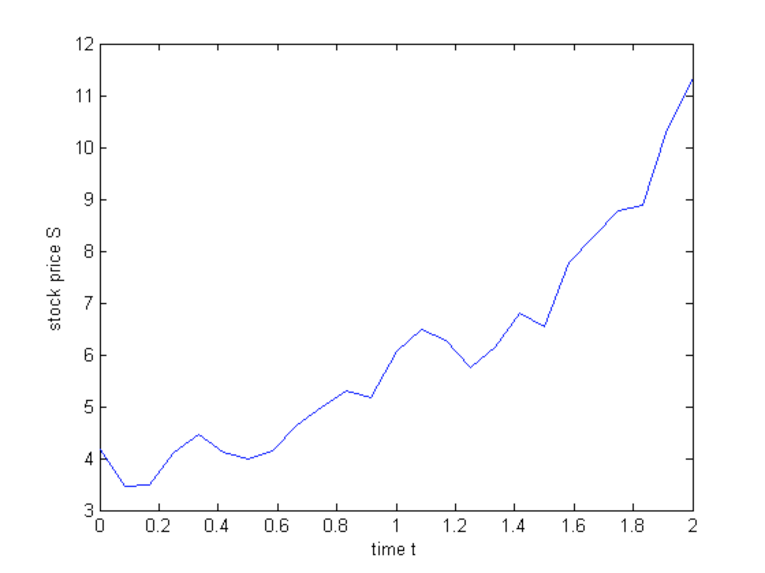
\includegraphics[totalheight=6cm]{pic/tu1}
	\caption{两年的股票走势}
\end{figure}

从图中我们可以看出,合同的价值是一个计息期比计息期要低,在每个实施日前一刻到达本记息期内的最大值,在实施日实施利息后,合同的价值明显的比上一个记息期要低的多,这是因为在给予一定的收益率后,合同的内在价值变小了的原因,虽然每次实施日不一定都能够得到最高的收益率,但是毕竟是少了1次得到收益率的机会了。


%==========================正文部分结束=================================
 	\backmatter

  \addcontentsline{toc}{chapter}{参考文献}
  \chaptermark{参考文献}
  \bibliography{data/tjbib}

  %附录部分
  \chapter*{附\quad录}
\chaptermark{附录}
\addcontentsline{toc}{chapter}{附录}
\songti \wuhao 宋体\quad 五号
  %谢辞部分
  \chapter*{\centerline{谢\quad辞}}
\chaptermark{谢辞}
\addcontentsline{toc}{chapter}{谢辞}

\vspace{2em}

\songti \wuhao 宋体 \quad 五号(略)



\end{document}